%\documentclass[12pt,notitlepage]{article}
\documentclass[a4paper,12pt]{article}
\usepackage[utf8]{inputenc}
\usepackage{graphicx}
\usepackage{verbatim}
\usepackage{amsthm}
\usepackage{amssymb}
\usepackage{pdfpages}
\usepackage{amsmath}
\usepackage{tikzsymbols}
\usetikzlibrary{arrows}
\usetikzlibrary{3d}
\newcommand{\midarrow}{\tikz \draw[-triangle 90] (0,0) -- +(.1,0);}
\pgfdeclarelayer{bg}    % declare background layer
\pgfsetlayers{bg,main}  % set the order of the layers (main is the standard layer)
\usepackage{mwe}
\usetikzlibrary{decorations.pathreplacing}
\usetikzlibrary{shapes}
\usepackage{mathtools}
\usepackage{enumitem}
\DeclarePairedDelimiter\ceil{\lceil}{\rceil}
\DeclarePairedDelimiter\floor{\lfloor}{\rfloor}
\usepackage{subcaption}

\usepackage{hyperref}
%\usepackage[T1]{fontenc}
\usepackage{url}
\usepackage{lipsum}
\usepackage{array}
\usepackage{multirow}
\usepackage{float}
\usepackage{lscape}
\usepackage{colortbl}
\newcolumntype{P}[1]{>{\centering\arraybackslash}p{#1}}
\usepackage[nottoc,numbib]{tocbibind}
\usepackage{fancyhdr}
\usepackage{hhline}
\usepackage[printonlyused]{acronym}
\usepackage{footmisc}

%\usepackage{txfonts}
\usepackage{lipsum,etoolbox}% http://ctan.org/pkg/{lipsum,etoolbox}
\usepackage{caption}
\usepackage{subcaption}
\usepackage{setspace}

\usepackage{algorithm}
\usepackage[noend]{algpseudocode}

\makeatletter
\def\BState{\State\hskip-\ALG@thistlm}
\makeatother

\usepackage{minted}

\definecolor{black}{RGB}{0,0,0}

\usepackage{fancyvrb}

\usepackage{geometry}
\geometry{
	a4paper,
	total={170mm,257mm},
	right=3cm,
	left=3cm,
	top=3cm,
	bottom=3cm
}



\makeatletter
\DeclareRobustCommand{\rvdots}{%
	\vbox{
		\baselineskip4\p@\lineskiplimit\z@
		\kern-\p@
		\hbox{.}\hbox{.}\hbox{.}
}}
\makeatother
\usepackage{titlesec}
\usepackage{hyperref}
\titleclass{\subsubsubsection}{straight}[\subsection]

\newcounter{subsubsubsection}[subsubsection]
\renewcommand\thesubsubsubsection{\thesubsubsection.\arabic{subsubsubsection}}
\renewcommand\theparagraph{\thesubsubsubsection.\arabic{paragraph}} % optional; useful if paragraphs are to be numbered

\titleformat{\subsubsubsection}
{\normalfont\normalsize\bfseries}{\thesubsubsubsection}{1em}{}
\titlespacing*{\subsubsubsection}
{0pt}{3.25ex plus 1ex minus .2ex}{1.5ex plus .2ex}

\makeatletter
\renewcommand\paragraph{\@startsection{paragraph}{5}{\z@}%
	{3.25ex \@plus1ex \@minus.2ex}%
	{-1em}%
	{\normalfont\normalsize\bfseries}}
\renewcommand\subparagraph{\@startsection{subparagraph}{6}{\parindent}%
	{3.25ex \@plus1ex \@minus .2ex}%
	{-1em}%
	{\normalfont\normalsize\bfseries}}
\def\toclevel@subsubsubsection{4}
\def\toclevel@paragraph{5}
\def\toclevel@paragraph{6}
\def\l@subsubsubsection{\@dottedtocline{4}{7em}{4em}}
\def\l@paragraph{\@dottedtocline{5}{10em}{5em}}
\def\l@subparagraph{\@dottedtocline{6}{14em}{6em}}
\makeatother
\newcommand*\circled[1]{\tikz[baseline=(char.base)]{
		\node[shape=circle,draw,inner sep=2pt] (char) {#1};}}


\setcounter{secnumdepth}{4}
\setcounter{tocdepth}{4}
\newcommand{\und}{\underline{\hspace{.10in}}}
\begin{document}
	\begin{titlepage}
		\begin{center}
			\vspace*{9em}
			\Huge 
			MH4921\\ Supervised Independent Study II\\
			\vspace*{4em}
			\LARGE
			\textbf{Linux Firewall Lab}\\		
			\vspace{4em}
			\textbf{Brandon Goh Wen Heng}\\
			\vspace*{4em}
			Academic Year 2018/19
			\vfill
		\end{center}
	\end{titlepage}
	
	\pagenumbering{roman}
	\tableofcontents
	\newpage
	\pagenumbering{arabic}
	\section{Introduction}
	Firewalls are commonly used to block traffic, as evident in enterprises and academic institutions where applications and sites are blocked to prevent distractions or illegal traffic from occurring within the networks. There are multiple types of firewall but this lab will focus on two types, the \textit{packet filter} and the application firewall.\\\\Packet filters act by inspecting the packets and if it matches any of the firewall rules, the packets are forwarded or dropped. Packet filters are mostly \textit{stateless}, in that the packets are filtered based on the information encoded in the individual packets and not based on the data stream. Packet filters may use a combination of the packet's source and destination address, protocol and port numbers among many fields.\\\\Application firewalls such as web proxies work at the application layer where the data of the packet is analysed. This method is primarily used for egress filtering of web traffic.
\section{Overview}
This lab will aim to bring insights on how firewalls work by making use of a firewall software and a simplified packet filtering firewall. The first three sections will look at how the packet filtering firewall \texttt{ufw} works and the counter measures that could be taken to evade this type of filtering.\\\\The last two sections of this lab will detail how access to websites can be controlled via a web proxy named \texttt{squid}, a type of application firewall. It will show how this type of firewall can be used to circumvent packet filtering firewalls. Also, \texttt{squid} can modify the contents of the displayed web page, using a method known as URL rewriting/redirection. The demonstration defaces the NTU home page on the local computer, elaborated in great detail at a later chapter of this report. 
\section{Exploration}
\subsection{Virtual Machine (VM) Configuration}
The firewall that will be used later needs to have its configuration modified as its default firewall policy drops all incoming packets. To change it, the default policy file \texttt{/etc/default/ufw} is opened and the following line is modified.\\\\
\texttt{DEFAULT\_INPUT\_POLICY = `DROP'} $\rightarrow$ \texttt{DEFAULT\_INPUT\_POLICY = `ACCEPT'}
\subsection{Using Firewalls}
Linux distributions have a built in kernel firewall tool named \texttt{iptables}. The front-end alternative that is more user-friendly is \texttt{ufw}. By using \texttt{ufw}, it can be used to create a personal firewall for the system but alternative means are more efficient when configuring firewalls for larger networks. For this task, the following are attempted.
\begin{itemize}
\item Prevent Machine A from executing \texttt{Telnet} to Machine B
\item Prevent Machine B from executing \texttt{Telnet} to Machine A
\item Prevent Machine A from visiting an external website. (Note that some websites have multiple IP addresses)
\end{itemize}
The manipulation of the firewall is performed on machine A while the firewall on machine B is untouched and left at the default setting.

\begin{figure}[H]
\centering
\begin{tikzpicture}			

\draw[fill=blue!10] (-5.15,2.15) rectangle (-3.85,1.25);
\draw (-5.3,2.3) rectangle (-3.7,1.1);
\draw (-4.1,1.1) rectangle (-4.9,0.6);
\draw (-5.1,0.75) -- (-5.5,0.4);
\draw (-3.9,0.75) -- (-3.5,0.4);
\draw (-5.5,0.4) -- (-3.5,0.4);
\draw (-5.1,0.75) -- (-4.9,0.75);
\draw (-3.9,0.75) -- (-4.1,0.75);
\draw (-4.5,-0.3) node[text width=3cm, align=center]{Machine A};

	\draw[fill=red!10] (3.05,2.15) rectangle (4.35,1.25);
\draw (2.9,2.3) rectangle (4.5,1.1);
\draw (4.1,1.1) rectangle (3.3,0.6);
\draw (3.1,0.75) -- (2.7,0.4);
\draw (4.3,0.75) -- (4.7,0.4);
\draw (2.7,0.4) -- (4.7,0.4);
\draw (3.1,0.75) -- (3.3,0.75);
\draw (4.3,0.75) -- (4.1,0.75);
\draw (3.64 ,-0.3) node[text width=4.5cm, align=center]{Machine B};

\draw(-1.4,1.35) node{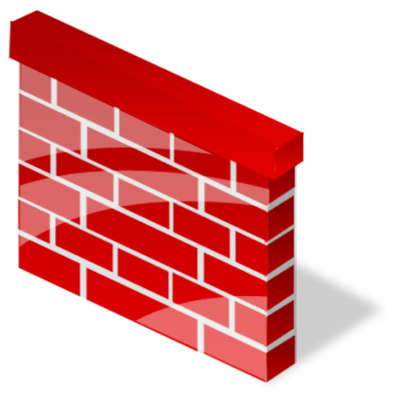
\includegraphics[width=0.14\linewidth]{firewall.png}};

\draw[rounded corners=8pt] (-6,2.65) rectangle (-0.4,-0.9);
\draw[rounded corners=8pt] (2,2.65) rectangle (5.2,-0.9);

\draw[->,line width=0.5mm](-3.7,1.6) -- (-2.34,1.6);
\draw[red,line width=0.8mm](-2.82,1.4) -- (-3.22,1.8);
\draw[red,line width=0.8mm](-2.82,1.8) -- (-3.22,1.4);

\draw[->,line width=0.5mm](2.9,1.3) -- (-0.91,1.3);
\draw[red,line width=0.8mm](0.8,1.1) -- (1.2,1.5);
\draw[red,line width=0.8mm](0.8,1.5) -- (1.2,1.1);
	\end{tikzpicture}
\caption{Firewall Setup}
\label{fig:Firewall}
\end{figure}
\begin{enumerate}
\item To prevent Machine A from executing \texttt{Telnet} to Machine B, it is known that Telnet uses (TCP) port 23. Furthermore from the ``Remote DNS Attack Lab'', source ports are randomised to prevent common ports from being hacked. Therefore, the firewall must block the destination ports instead.\\\\Using \texttt{ufw}, there are multiple ways to block \texttt{Telnet} from being used from Machine A to Machine B. Below are two different methods that can be used to block outgoing \texttt{Telnet} packets.
\begin{verbatim}
$ ufw deny out to any port 23
$ ufw reject out telnet
\end{verbatim}
The commands \texttt{ufw disable} and \texttt{ufw enable} have to be used to force the firewall to enforce the new firewall rules. (*Note: because Telnet is a well known program that uses TCP port 23, the second line of code can be used. Otherwise the first line is more straightforward and direct.)\\\\
Blocking \texttt{Telnet} on the firewall level will prevent the packets from reaching the intended destination and eventually force \texttt{Telnet} to timeout, as shown in the figure below.


\begin{figure}[H]
    \centering
\begin{subfigure}[H]{0.45\textwidth}
\centering
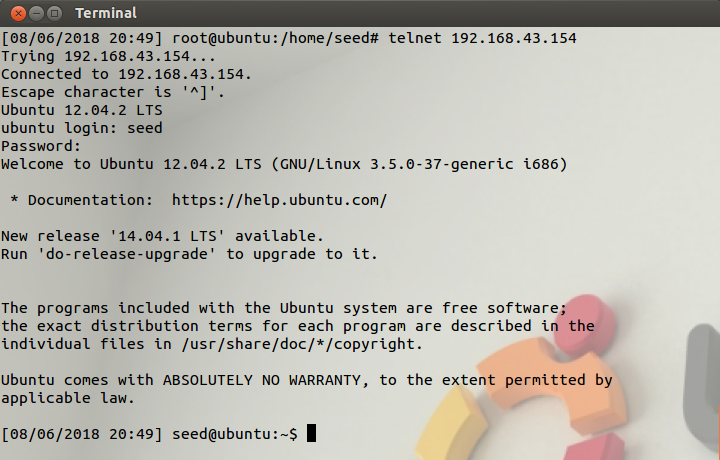
\includegraphics[width=1\linewidth]{telnetmachB}
\caption{Before Firewall Rule}
\label{fig:MachB}
\end{subfigure}
~
\begin{subfigure}[H]{0.45\textwidth}
\centering
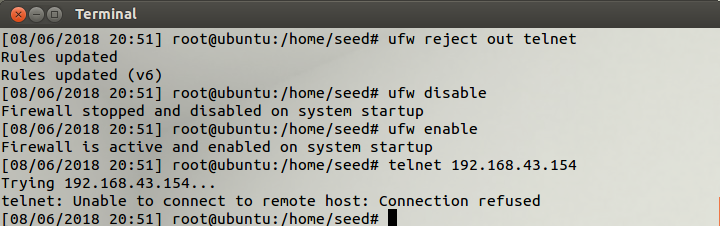
\includegraphics[width=1\linewidth]{telnetmachBdenied}
\caption{After Firewall Rule}
\label{fig:MachBDenied}
\end{subfigure}
    \caption{Prevent \texttt{Telnet} to External Host}
    %\label{fig:lengthdetermination}
\end{figure}

\item To prevent Machine B from executing \texttt{Telnet} to Machine A, it is the same as the previous. However, the direction of the packet flow has been swapped. Due to this, the direction when writing the commands is of importance in determining whether the blocking is successful.\\\\Again, there are two ways of blocking which is provided below.
\begin{verbatim}
$ sudo ufw deny in to any port 23
$ sudo ufw reject in telnet
\end{verbatim}
Again, the commands \texttt{ufw disable} and \texttt{ufw enable} have to be used to force the firewall to enforce the new firewall rules. Executing \texttt{Telnet} from machine B will yield the same timeout message.

\begin{figure}[H]
    \centering
\begin{subfigure}[H]{1\textwidth}
\centering
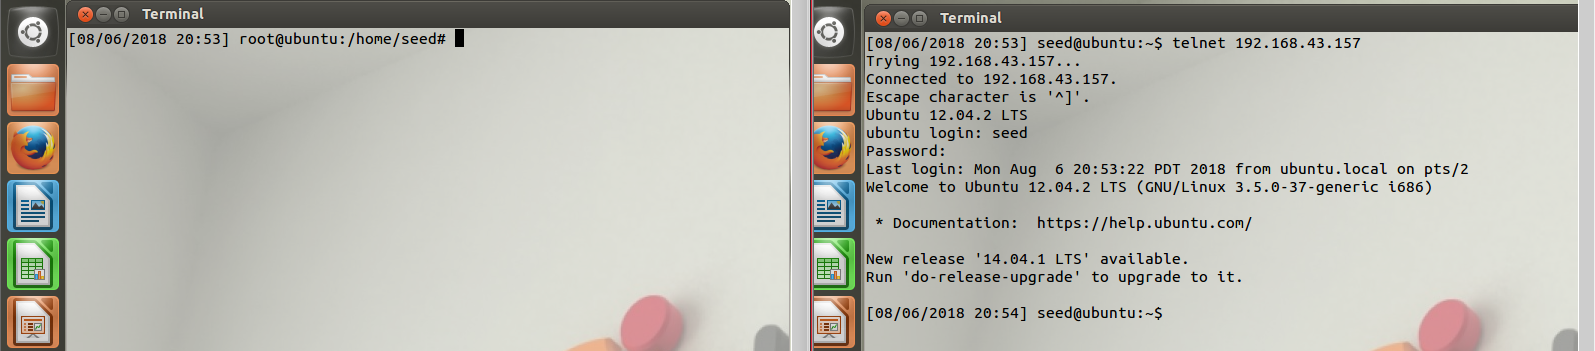
\includegraphics[width=1\linewidth]{telnetmachA}
\caption{Before Firewall Rule}
\label{fig:MachA}
\end{subfigure}
\vspace{1em}
\begin{subfigure}[H]{1\textwidth}
\centering
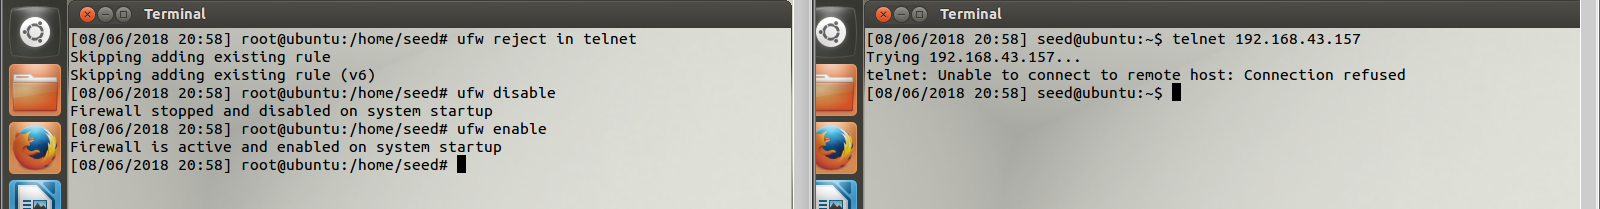
\includegraphics[width=1\linewidth]{telnetmachAdenied}
\caption{After Firewall Rule}
\label{fig:MachADenied}
\end{subfigure}
    \caption{Prevent \texttt{Telnet} to Current Host}
    %\label{fig:lengthdetermination}
\end{figure}
\item To prevent machine A from accessing a website, we can use \texttt{ufw} to perform the filtering. However, \texttt{ufw} is not able to block hostnames and as such the IP address must be known. In this task, the site \texttt{www.ntu.edu.sg} will be blocked. To find out the IP address of the site, the command \texttt{dig} is sufficient to reveal the A records of the hostname.\\\\To block (non-secured) websites, TCP port 80 must be blocked (443 for secured websites). Since the port numbers are directed to the server-side, outgoing packets are filtered. To do so, the following line can be used to block the site.
\begin{verbatim}
$ sudo ufw deny out to 155.69.7.173 port 80
\end{verbatim}
The firewall is restarted to effect the changes and refreshing the site will now show that the connection to the website has timed out and cannot be restored.
\begin{figure}[H]
    \centering
\begin{subfigure}[H]{0.45\textwidth}
\centering
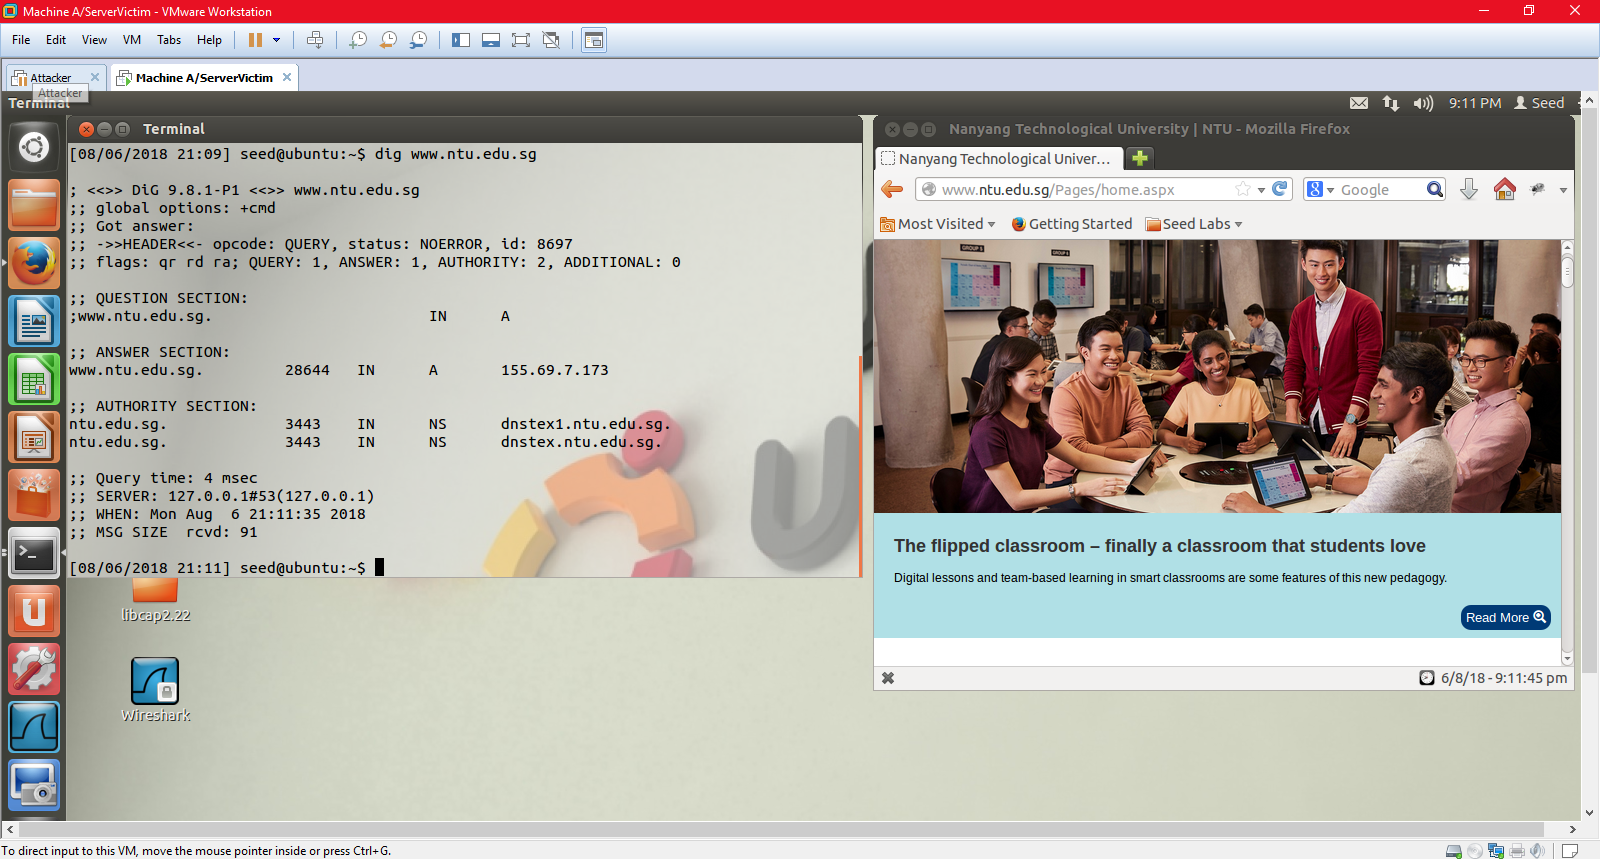
\includegraphics[width=1\linewidth]{webAaccess}
\caption{Before Firewall Rule}
\label{fig:WebA}
\end{subfigure}
~
\begin{subfigure}[H]{0.45\textwidth}
\centering
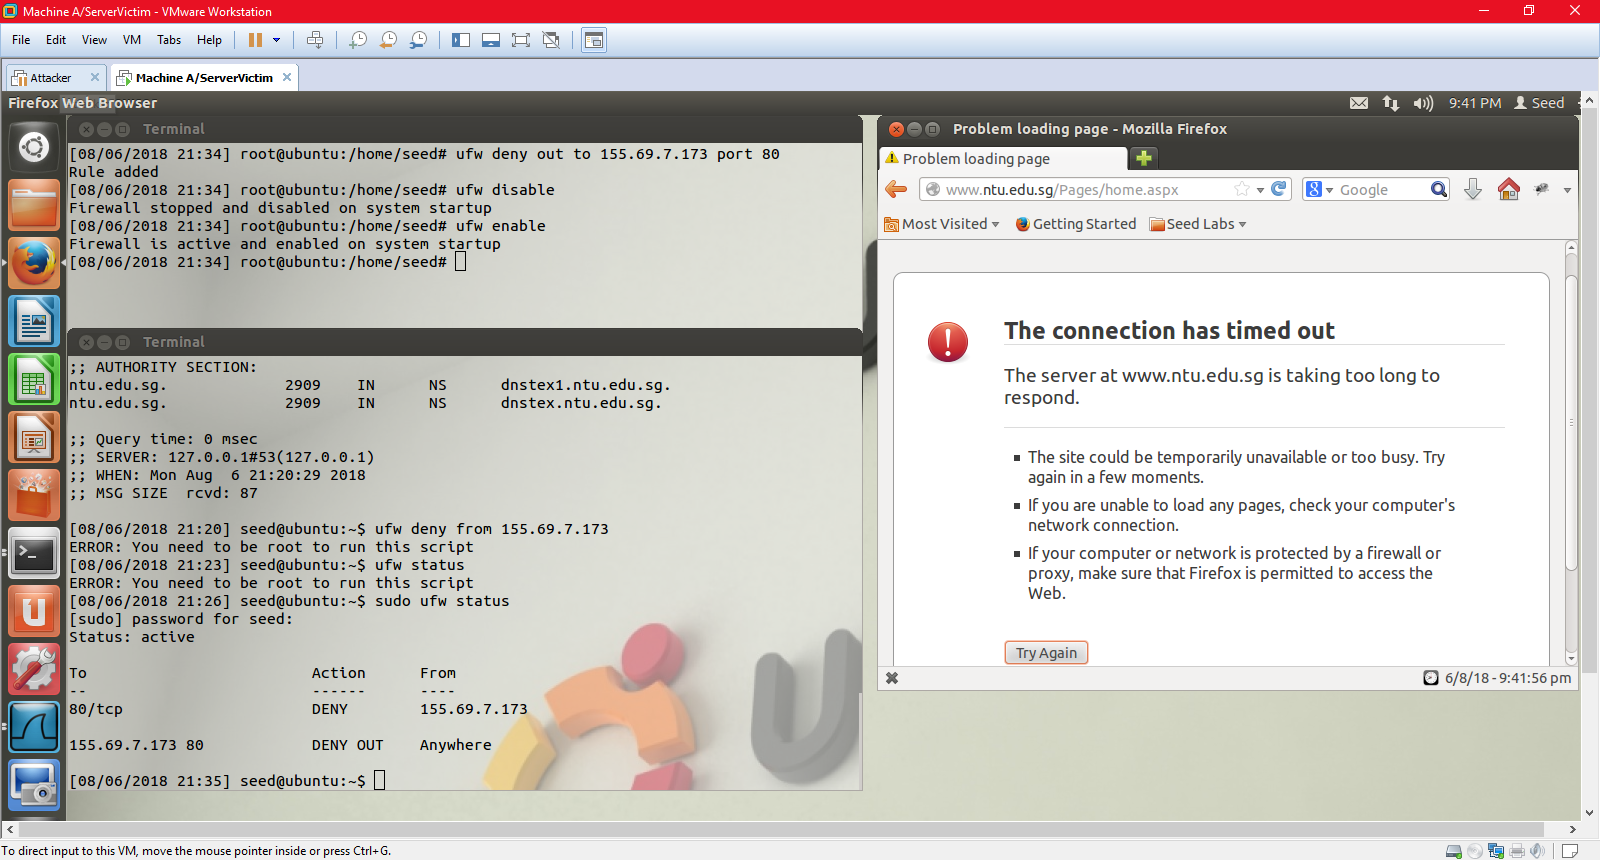
\includegraphics[width=1\linewidth]{webAaccessdenied}
\caption{After Firewall Rule}
\label{fig:WebADenied}
\end{subfigure}
    \caption{Block Website Access}
    %\label{fig:lengthdetermination}
\end{figure}
\end{enumerate}

\noindent The \texttt{ufw} firewall uses packet filtering to inspect incoming and outgoing packets and to enforce the various policies configured by the administrator. As packet processing is performed in the kernel, as can be demonstrated in the ``Packet Sniffing and Spoofing Lab'', the filtering must also be performed within the kernel. However, using the \textit{Loadable Kernel Module} (\texttt{LKM}) and \texttt{Netfilter}, the kernel need not be rebuilt to manipulate packets. 
\\\\\noindent
\texttt{LKM} extends the functionalities of the kernel by allowing administrators to add modules without rebuilding the kernel or rebooting the computer. To process the packets and to block it, the module must be integrated into the packet processing path, which was not easily implemented before \texttt{Netfilter}.\\\\
Netfilter allows the manipulation of packets by allowing administrators to implement hooks into the Linux kernel. These hooks exists in various places and programs (within LKM) and gets invoked when packets pass through.
\\\\\textbf{Question 1:}\\
What types of hooks does \texttt{Netfilter} support and what can be done using these hooks? Draw also a diagram to show how packets flow through these hooks.\\\\
\textbf{Answer 1:}\\
There are a total of \texttt{5} hooks that can be used with \texttt{Netfilter} and these hooks can be found in the header definition of \texttt{netfilter\_ipv4.h} and \texttt{netfilter\_ipv6.h}, both located in the folder \texttt{/usr/include/linux} (If \texttt{gcc} is installed). The various hooks, together with its description are listed in the table below.

\begin{table}[H]
\footnotesize
\begin{tabular}{l|l|l}

{\underline{IPv4 Hooks}}   & {\underline{IPv6 Hooks}}    & {\underline{Description}}  \\\hline                                                                                                                                       NF\_IP\_PRE\_ROUTING  & NF\_IP6\_PRE\_ROUTING  & \begin{tabular}[c]{@{}l@{}}This hook is triggered when packets \\ enter into the network stack. After \\ that, the packet is routed or dropped \\ depending on the destination of the \\ packet.\end{tabular} \\\hline
NF\_IP\_LOCAL\_IN     & NF\_IP6\_LOCAL\_IN     & \begin{tabular}[c]{@{}l@{}}This hook is triggered when the \\ packet is designated for the local \\ system.\end{tabular} \\\hline
NF\_IP\_FORWARD       & NF\_IP6\_FORWARD       & \begin{tabular}[c]{@{}l@{}}This hook is triggered when the \\ packet is designed to be routed out to \\ another system.\end{tabular} \\\hline
NF\_IP\_LOCAL\_OUT    & NF\_IP6\_LOCAL\_OUT    & \begin{tabular}[c]{@{}l@{}}This hook is triggered when packets \\ are created locally and are outgoing \\ to the network.\end{tabular} \\\hline
NF\_IP\_POST\_ROUTING & NF\_IP6\_POST\_ROUTING & \begin{tabular}[c]{@{}l@{}}This hook is triggered just before \\ packets are to be sent out the \\ physical wire. \end{tabular}  
\end{tabular}
\caption{Table of \texttt{Netfilter} Hooks}
\label{tab:nethook}
\end{table}
\noindent *For newer kernel versions, the prefix \texttt{NF\_IP} has been changed to \texttt{NF\_INET}.\\\\The figure below depicts the different locations where the programs can hook onto the networking stack to manipulate the respective packets.
\begin{figure}[H]
	\centering
	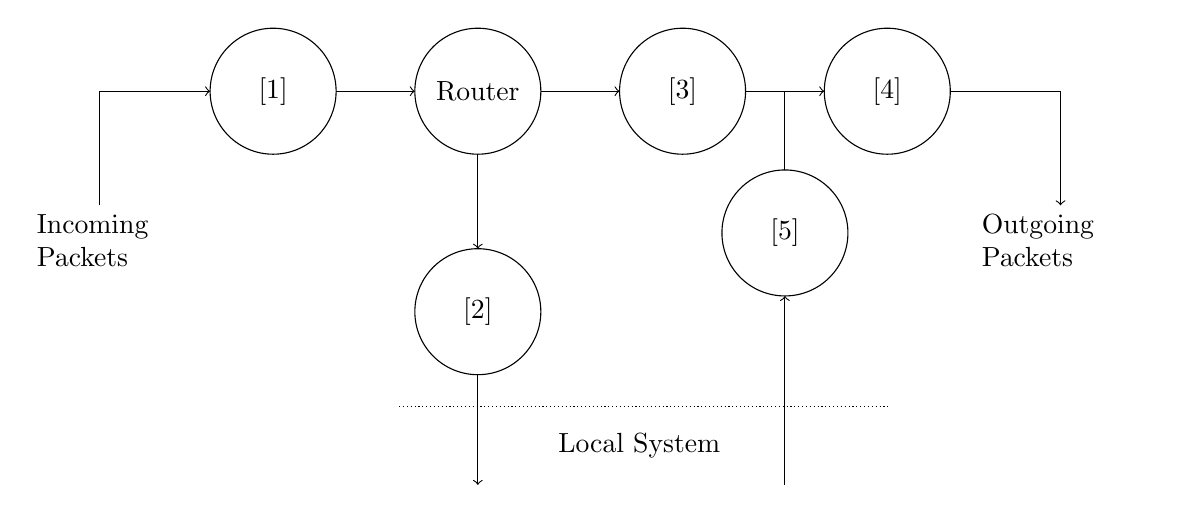
\begin{tikzpicture}	
	\draw(-2,-2) node[text width=2cm,yshift=0.1cm]{Incoming \\Packets};
	\draw[->] (-2.2,-1.45)--(-2.2,0) -- (-0.8,0);
\draw(0,0) circle (0.8cm)node {[1]};
\draw[->](0.8,0) -- (1.8,0);
\draw (2.6,0) circle (0.8cm) node{Router};
\draw[->](2.6,-0.8) -- (2.6,-2);
\draw(2.6,-2.8)circle(0.8cm)node{[2]};
\draw[->](2.6,-3.6)--(2.6,-5);
\draw[->] (3.4,0) -- (4.4,0);
\draw (5.2,0) circle(0.8cm) node{[3]};
\draw[->] (6,0)-- (7,0);
\draw(7.8,0) circle(0.8cm) node{[4]};
\draw[->](8.6,0)-- (10,0)--(10,-1.45);
\draw(10,-2) node[text width=2cm,yshift=0.1cm]{Outgoing \\Packets};
\draw(6.5,0)--(6.5,-1);
\draw(6.5,-1.8)circle(0.8cm)node{[5]};
\draw[->](6.5,-5)--(6.5,-2.6);
\draw[densely dotted](1.6,-4) -- (7.8,-4);
\draw(4.05,-4.5)node[xshift=0.6cm]{Local System};
		\end{tikzpicture}
		\flushleft
[1]: NF\_IP\_PRE\_ROUTING\\
{[2]}: NF\_IP\_LOCAL\_IN\\
{[3]}: NF\_IP\_FORWARD\\
{[4]}: NF\_IP\_POST\_ROUTING\\
{[5]}: NF\_IP\_LOCAL\_OUT
	\caption{\texttt{Netfilter} System}
	\label{fig:NetSys}
\end{figure}
\noindent \textbf{Question 2:}\\
Where should a hook be placed for ingress and egress filtering?\\\\
\textbf{Answer 2:}\\
Ingress filtering is a technique to prevent suspicious traffic from entering the internal network. Ingress filtering checks for the validity of packets by analysing its source addresses to ensure that the IP address used does not originate within the network or any private addresses such as multicast. Therefore, an ingress filtering hook should be placed at NF\_IP\_PRE\_ROUTING, before it proceeds to any part of the network.\\\\For egress filtering, it is the opposite of ingress filtering. It checks for outgoing packets and prevents data from flowing out, such as malicious packets containing spyware. In this case, egress filtering must be hooked to NF\_IP\_POST\_ROUTING.\\\\
\textbf{Question 3:}\\
Can packets be modified using \texttt{Netfilter}?\\\\
\textbf{Answer 3:}\\
While \texttt{Netfilter} is primarily used for analysing incoming, outgoing packets and to block where required based on the firewall policy, the user can write programs (within LKM) that hook onto \texttt{Netfilter} and use it to modify packets instead.
\subsection{Optional: Implementing Packet Filtering Module}
A firewall should support dynamic configurations and be able to dynamically change firewall policies. The configuration tool runs in the user space, but the data has to be sent to the kernel space where the packet filtering module (LKM) can obtain the data. These data must reside in the kernel memory instead of a file due to performance issues. This involves interactions between a user-level program and the kernel module.\\\\
Using sample code provided by Paul Kiddie\footnote{\url{https://www.paulkiddie.com/2009/10/creating-a-simple-hello-world-netfilter-module/}}, the code is extended to drop IPv4 ICMP (ping) packets instead of all packets. Before proceeding, there are multiple ways to process the packets using our module. These definitions are located inside \texttt{netfilter.h}.
\begin{enumerate}
\itemsep0em
\item NF\_DROP: Drop packet.
\item NF\_ACCEPT: Accept packet and process through network chain.
\item NF\_STOLEN: Ownership of packet transferred to hook and \texttt{Netfilter} will not process the packet further.
\item NF\_QUEUE: Get \texttt{Netfilter} to queue the packet for userspace.
\item NF\_REPEAT: Call the hook again.
\item NF\_STOP: Accept packet and stop further processing along network chain.
\end{enumerate}
The kernel module needs to be compiled via a \texttt{Makefile}. Both the packet filtering module code and the \texttt{makefile} code have been attached to \hyperref[ch:AppA]{Appendix A}. It also interesting to note that when compiling the file via \texttt{Makefile}, the module libraries are located in \texttt{/lib/modules/\$(shell uname -r)/build/include}. This is in contrast to normal compilation using \texttt{gcc}, where the libraries are located in the folder \texttt{/usr/include}.\\\\When compiling code, it is best to ensure that there are no warnings that appear as these errors may crash the system when the module is loaded into the kernel.


\begin{figure}[H]
\centering
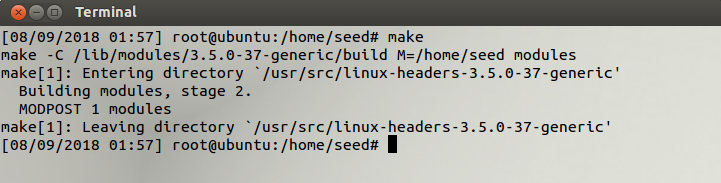
\includegraphics[width=0.7\linewidth]{makecomplete}
\caption{No errors during \texttt{make}}
\label{fig:makecomplete}
\end{figure}


\noindent To add the compiled program into the kernel, the following command is used.
\begin{verbatim}
$ sudo insmod pfm.ko
\end{verbatim}
\noindent The code provided is compiled and further extended to only drop IPv4 ICMP packets. These programs are loaded into the kernel with names \texttt{pfm.ko} and \texttt{pfm2.ko} respectively. To remove the kernel modules and to display the kernel log, the following two lines can be used.
\begin{verbatim}
$ sudo rmmod pfm.ko
$ dmesg | tail -10 //Where 10 stands for the last x lines displayed
\end{verbatim}
\noindent Looking at the figures below, both \texttt{ping} and \texttt{Telnet} are used to show the different types of packets that are accepted or dropped.
\\
	\begin{figure}[H]
	\centering
		\begin{subfigure}[H]{0.45\textwidth}
			\centering
			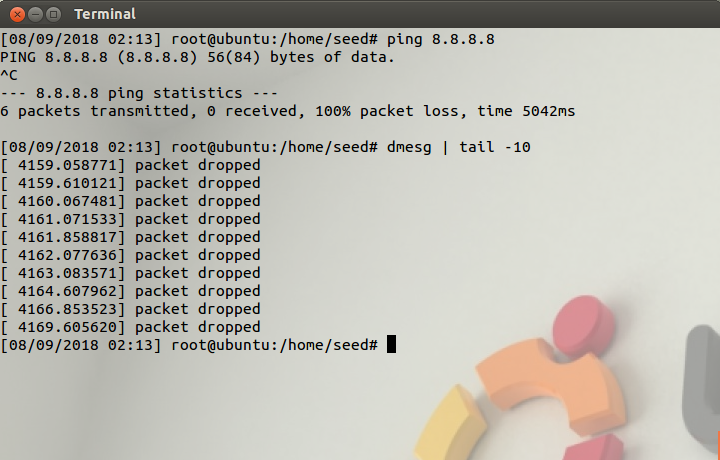
\includegraphics[width=1\linewidth]{pingdropall}
			\caption{Dropped \texttt{ping} Packets}
			\label{fig:pingdropall}
		\end{subfigure}
	~
		\begin{subfigure}{0.45\textwidth}
			\centering
			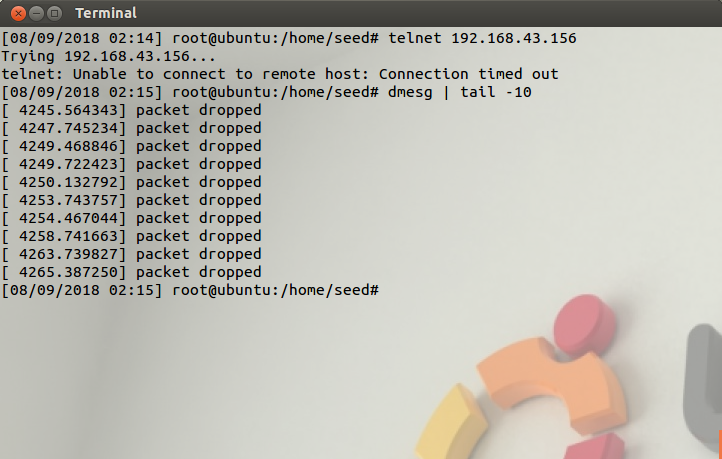
\includegraphics[width=1\linewidth]{telnetdropall}
			\caption{Dropped \texttt{Telnet} Packets}
			\label{fig:telnetdropall}
		\end{subfigure}
		\caption{All Packets Dropped}
	\end{figure}
	\begin{figure}[H]
	\centering
		\begin{subfigure}{0.45\textwidth}
			\centering
			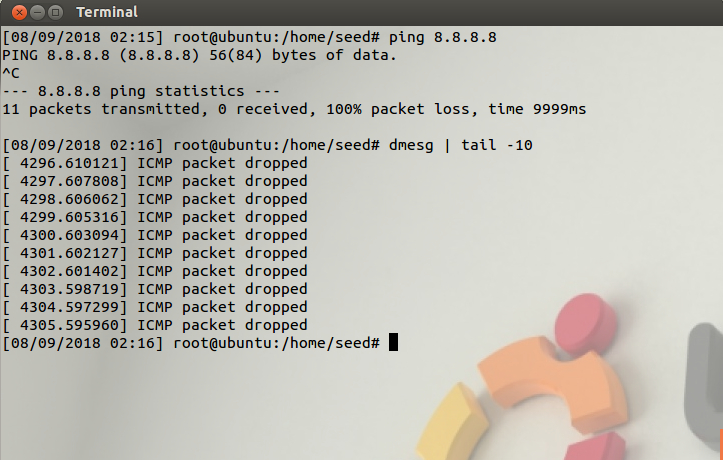
\includegraphics[width=1\linewidth]{pingicmpdrop}
			\caption{Dropped \texttt{ping} Packets}
			\label{fig:icmppingdrop}
		\end{subfigure}
		~
		\begin{subfigure}[H]{0.45\textwidth}
			\centering
			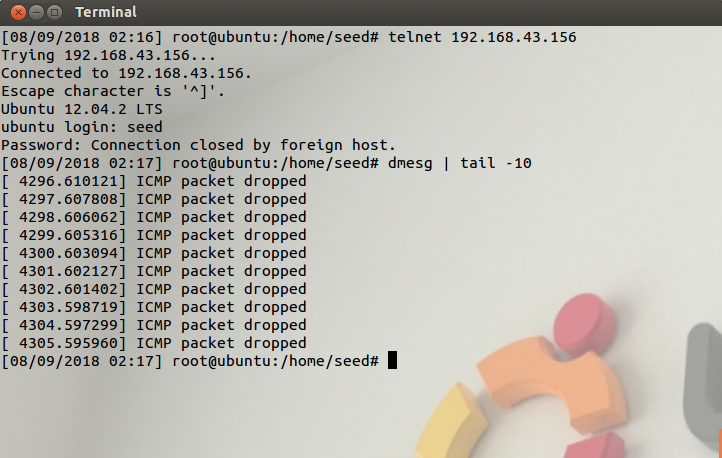
\includegraphics[width=1\linewidth]{telneticmpdrop}
			\caption{\texttt{Telnet} Packets Allowed}
			\label{fig:telneticmpdrop}
		\end{subfigure}
		\caption{Only ICMP Packets Dropped}
	\end{figure}
\noindent From the two figures above, all packets were dropped when the module was attached to the kernel, except for figure 8b. In can be seen that \texttt{Telnet} can be executed and the timestamp for the logs are for the dropped \texttt{ping} packets in figure 8a.
\subsection{Evading Egress Filtering}
Egress filtering is commonly used in companies and schools to restrict the use of certain services and applications. These firewalls inspect the destination IP addresses and port numbers of outgoing packets and dropped if any matches the firewall rules. Deep packet inspections are not performed on the packets due to performance reasons and therefore using the tunnelling mechanism, egress filtering can be bypassed.\\\\
Three VMs are setup to demonstrate this purpose. Machine A is behind a firewall while Machines B and C are outside of the firewall. The following firewall rules are also setup using \texttt{ufw} on Machine A as it is more convenient than re-writing the hook.
\begin{enumerate}
\itemsep0em
\item All outgoing traffic to external telnet servers are blocked. The \texttt{Telnet} server is run on Machine C and can be started using the command \texttt{sudo service openbsd-inetd start}.
\item All outgoing traffic to \texttt{www.facebook.com} are blocked to emulate the restriction in companies/schools to prevent them from being distracted. As Facebook runs on 2 IP addresses, both are blocked (including its https variants). The following lines of code are run to ensure all IP addresses of Facebook are blocked.
\begin{verbatim}
$ sudo ufw deny out to 157.240.7.38 port 80
$ sudo ufw deny out to 157.240.7.38 port 443
$ sudo ufw deny out to 157.240.7.35 port 80
$ sudo ufw deny out to 157.240.7.35 port 443
$ sudo ufw disable
$ sudo ufw enable
\end{verbatim}
To check whether the implementation is successful, the browser can either have its cache cleared or perform a force refresh (\texttt{Ctrl+R}).
\end{enumerate}
\subsubsection{\texttt{Telnet} Bypass}
To bypass the firewall, a SSH tunnel between Machine A and B can be established. This will allow all telnet traffic to go through encrypted, evading any inspection. The following line establishes a SSH tunnel from the localhost's port 8000 Machine B and packets that exit Machine B's SSH port will be forwarded to Machine C.
\begin{verbatim}
$ ssh -L 8000:<Machine C IP>:23 seed@<Machine B IP>
\end{verbatim}
More details on the local and remote forwarding switches can be found on the \href{https://unix.stackexchange.com/questions/115897/whats-ssh-port-forwarding-and-whats-the-difference-between-ssh-local-and-remot}{Unix Stack Exchange}.

\begin{figure}[H]
\centering
\begin{tikzpicture}			

\draw[fill=blue!10] (-5.15,2.15) rectangle (-3.85,1.25);
\draw (-5.3,2.3) rectangle (-3.7,1.1);
\draw (-4.1,1.1) rectangle (-4.9,0.6);
\draw (-5.1,0.75) -- (-5.5,0.4);
\draw (-3.9,0.75) -- (-3.5,0.4);
\draw (-5.5,0.4) -- (-3.5,0.4);
\draw (-5.1,0.75) -- (-4.9,0.75);
\draw (-3.9,0.75) -- (-4.1,0.75);
\draw (-4.5,-0.3) node[text width=3cm, align=center]{Machine A};

	\draw[fill=red!10] (3.05,2.15) rectangle (4.35,1.25);
\draw (2.9,2.3) rectangle (4.5,1.1);
\draw (4.1,1.1) rectangle (3.3,0.6);
\draw (3.1,0.75) -- (2.7,0.4);
\draw (4.3,0.75) -- (4.7,0.4);
\draw (2.7,0.4) -- (4.7,0.4);
\draw (3.1,0.75) -- (3.3,0.75);
\draw (4.3,0.75) -- (4.1,0.75);
\draw (3.64 ,-0.3) node[text width=4.5cm, align=center]{Machine B};

	\draw[fill=yellow!10] (3.05,-0.85) rectangle (4.35,-1.75);
\draw (2.9,-0.7) rectangle (4.5,-1.9);
\draw (4.1,-1.9) rectangle (3.3,-2.4);
\draw (3.1,-2.25) -- (2.7,-2.6);
\draw (4.3,-2.25) -- (4.7,-2.6);
\draw (2.7,-2.6) -- (4.7,-2.6);
\draw (3.1,-2.25) -- (3.3,-2.25);
\draw (4.3,-2.25) -- (4.1,-2.25);
\draw (3.64 ,-3.3) node[text width=4.5cm, align=center]{Machine C};

\draw(-1.15,1.25) node{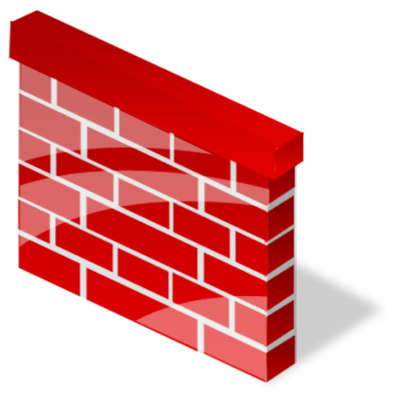
\includegraphics[width=0.20\linewidth,height=0.3\linewidth]{firewall.png}};

\draw[rounded corners=8pt] (-6,3.7) rectangle (-0,-0.9);
\draw[rounded corners=8pt] (2,2.65) rectangle (5.2,-3.9);

\draw[yellow,line width=0.5mm](-2.53,1.45) -- (-0.44,1.45);
\draw[line width=0.5mm](-3.7,1.45) -- (-2.53,1.45);
\draw[->,line width=0.5mm](-0.44,1.45) -- (2.9,1.45);
%\draw[red,line width=0.8mm](-2.82,1.2) -- (-3.22,1.6);
%\draw[red,line width=0.8mm](-2.82,1.6) -- (-3.22,1.2);
\draw[->,line width=0.5mm,bend right](2.9,1.35) to (2.9,-1.1);
\draw[<-,line width=0.5mm](2.9,-1.3) -- (-0.46,-0.06);
\draw[->,line width=0.5mm](-3.7,1.3) -- (-2.53,0.8);

\draw[red,line width=0.8mm](0.8,-0.77) -- (1.2,-0.37);
\draw[red,line width=0.8mm](0.8,-0.37) -- (1.2,-0.77);

\draw(-3.2,1.45)--(-3.2,3.8)node[yshift=0.2cm]{TCP port 8000};
\draw(1.3,1.45)--(1.3,3.8)node[yshift=0.2cm]{TCP port 22};
\draw(-3.2,1.10)--(-3.2,-2.1)node[yshift=-0.2cm]{TCP port 23};
\draw(-3.2,-1.8)-- (1.55,-1.8)--(1.55,-0.5)--(2.65,-0.5);
\draw(1.3,3)--(1.55,3)--(1.55,1.1)--(2.8,1.1);
	\end{tikzpicture}
	\flushleft
	Machine A has IP address 192.168.43.157\\Machine B has IP address 192.168.43.154\\Machine C has IP address 192.168.43.156
\caption{SSH Tunneling}
\label{fig:SSHTun}
\end{figure}

\noindent Once the SSH tunnel has been established, another Terminal window is opened. To connect to Machine C, we will force \texttt{Telnet} to use port 8000 since the packet will be forwarded to Machine C via the SSH tunnel.
\begin{verbatim}
$ telnet localhost 8000
\end{verbatim}
Using this method, Machine A can successfully be connected to Machine C via \texttt{Telnet}. The \texttt{ifconfig} is run to check whether the IP address of the connected system is correct and this is shown in the figure below.

\begin{figure}[H]
\centering
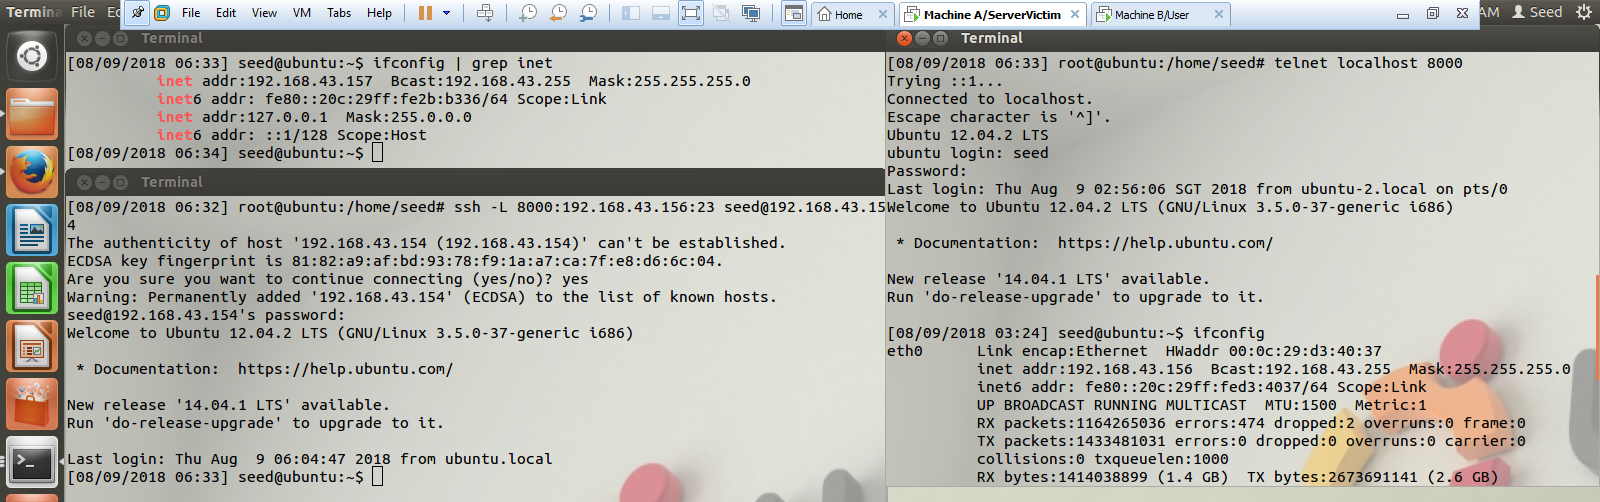
\includegraphics[width=1\linewidth]{telnetegressok}
\caption{Successfully Connected to Machine C}
\label{fig:telnetegressok}
\end{figure}
\noindent Wireshark is looked at and it can be seen that one cycle out from and back to Machine A includes
\begin{enumerate}
\itemsep0em
\item Sending an encrypted packet from Machine A to Machine B via SSH
\item Machine B sending \texttt{Telnet} data to Machine C
\item Machine C returns back \texttt{Telnet} acknowledgement data and packet
\item Machine B sends the data back to Machine A in an encrypted response packet via SSH
\end{enumerate}
Packet numbers 18 -- 22 in the Wireshark screen capture below show the corresponding interactions between all three machines to transfer data.
\begin{figure}[H]
\centering
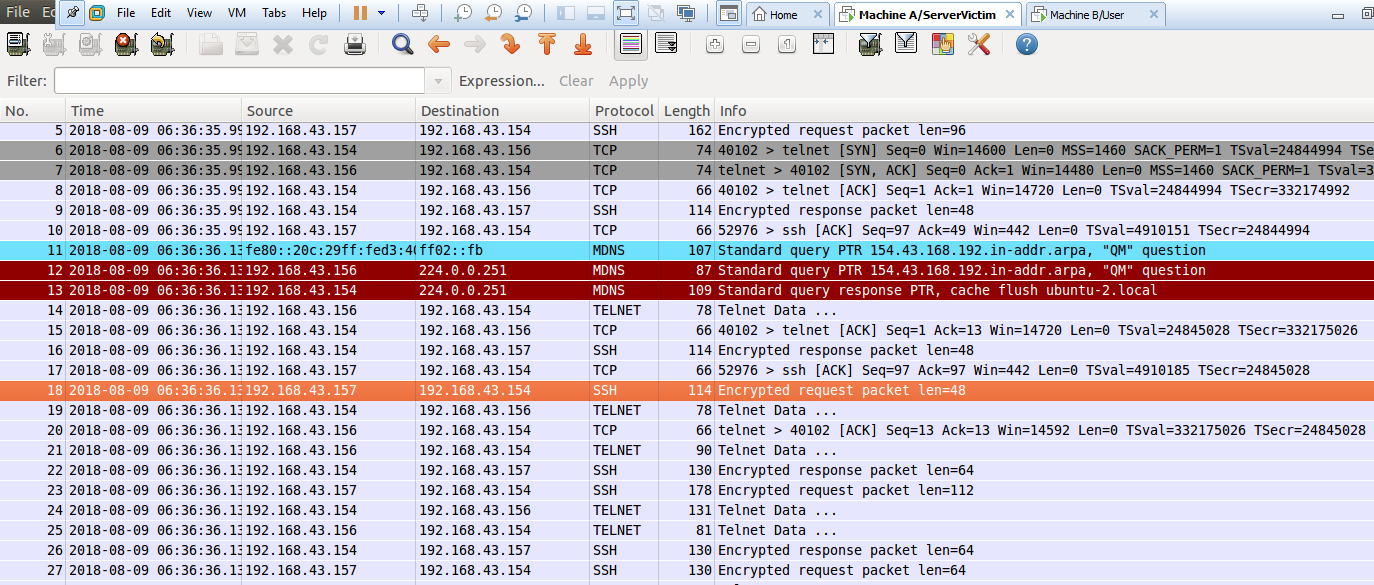
\includegraphics[width=1\linewidth]{wiresharkegress}
\caption{Wireshark Packet Flow}
\label{fig:wiresharkegress}
\end{figure}
\subsubsection{Facebook Bypass}
In this task, the same approach using static port forwarding can be used to bypass the firewall. However, dynamic port forwarding can also be used. Instead of requiring that the destination IP address and port number be specified, these can now be omitted. Using dynamic port forwarding only requires the source port and the intermediary IP address be specified, as the intermediary system will determine where it will forward based on the destination IP address encoded in the packet.\\\\The following command allows us to perform dynamic port forwarding using SSH.
\begin{verbatim}
$ ssh -D 9000 -C seed@<Machine B IP>
\end{verbatim}
The \texttt{-D} flag is used to specify that it is a dynamic port forwarding tunnel and the \texttt{-C} flag is used to force data compression.\\\\To make use of port 9000 SSH tunnel, the browser must also be configured to make use of it. To configure Firefox, navigate to \texttt{Edit > Preferences > Advanced > Network > Settings}. Under ``Manual proxy configuration'', SOCKS Host should be set to either \texttt{localhost} or 127.0.0.1, port set to 9000 and ``SOCKS v5'' selected. Under ``No Proxy for:'', the entries should be \texttt{localhost, 127.0.0.1}.
\begin{figure}[H]
\centering
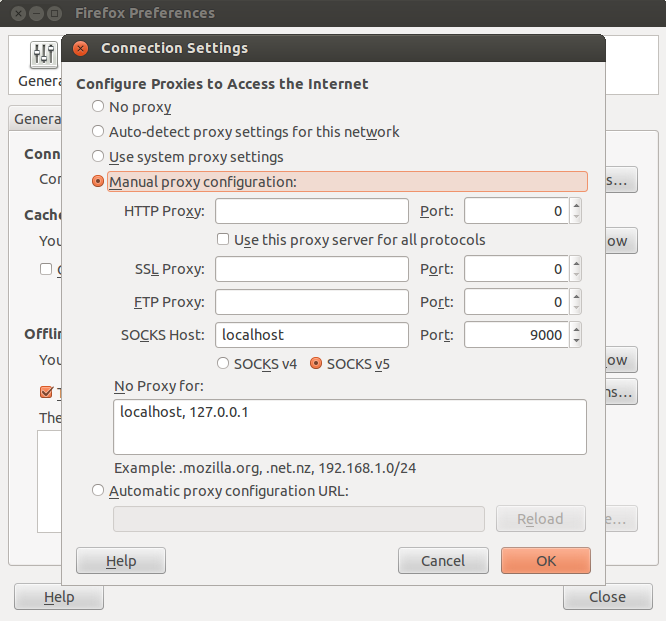
\includegraphics[width=0.7\linewidth]{FFConfig}
\caption{Firefox Configuration}
\label{fig:ffconfig}
\end{figure}

\noindent When the SSH tunnel is running in the background on a \texttt{Terminal} window, Facebook can be accessed normally via the browser. If the SSH tunnel is broken, Facebook will again be blocked due to the firewall (after removing the proxy settings).

\begin{figure}[H]
	\centering
		\begin{subfigure}[H]{0.8\textwidth}
			\centering
			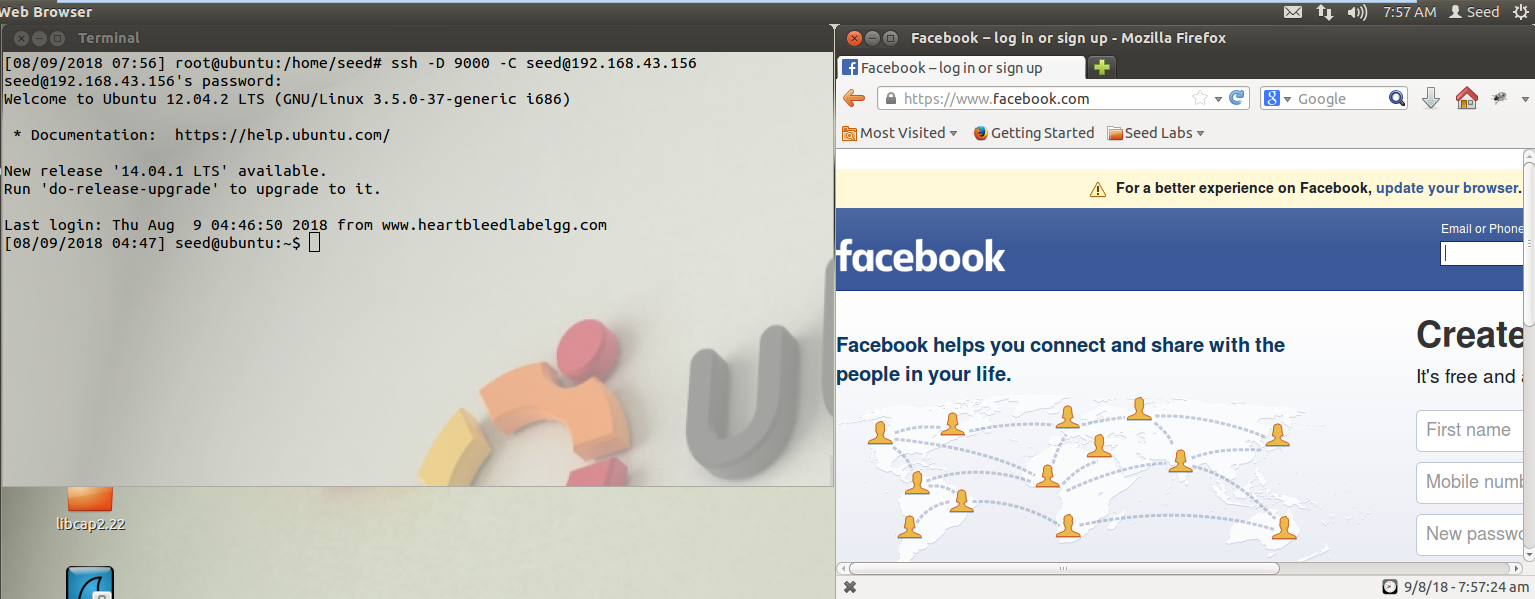
\includegraphics[width=1\linewidth]{facebookegressok}
			\caption{Accessing Facebook via SSH}
			\label{fig:FacebookSSH}
		\end{subfigure}
		\begin{subfigure}{0.8\textwidth}
			\centering
			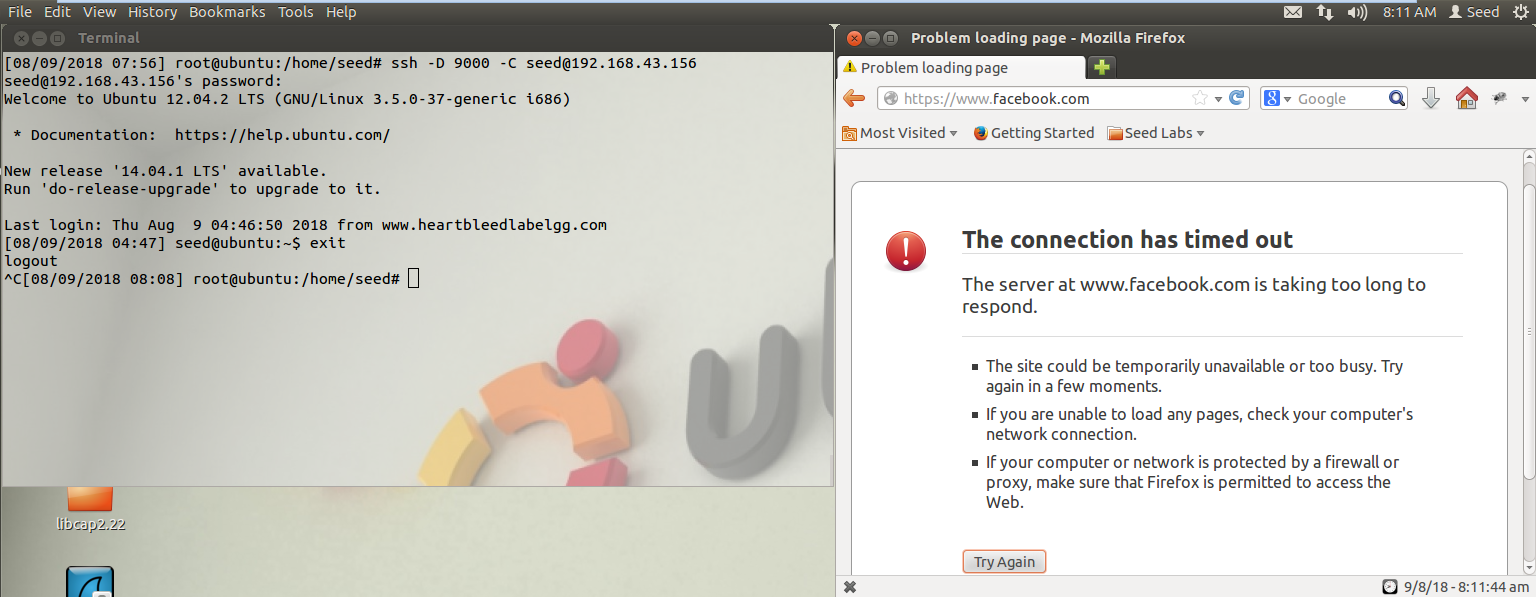
\includegraphics[width=1\linewidth]{facebooktimeout}
			\caption{Blocked Without SSH}
			\label{fig:FacebookBlock}
		\end{subfigure}
		\caption{Differences with SSH Tunnel}
	\end{figure}
\noindent Using Wireshark to analyse the transmitted packets, the same pattern is reflected as the previous task on \texttt{Telnet}. The data is transmitted to Machine C via SSH and it is then forwarded over to Facebook's servers (Client Hello). The server returns back the response to Machine C and it is forwarded back to Machine A via SSH.

\begin{figure}[H]
\centering
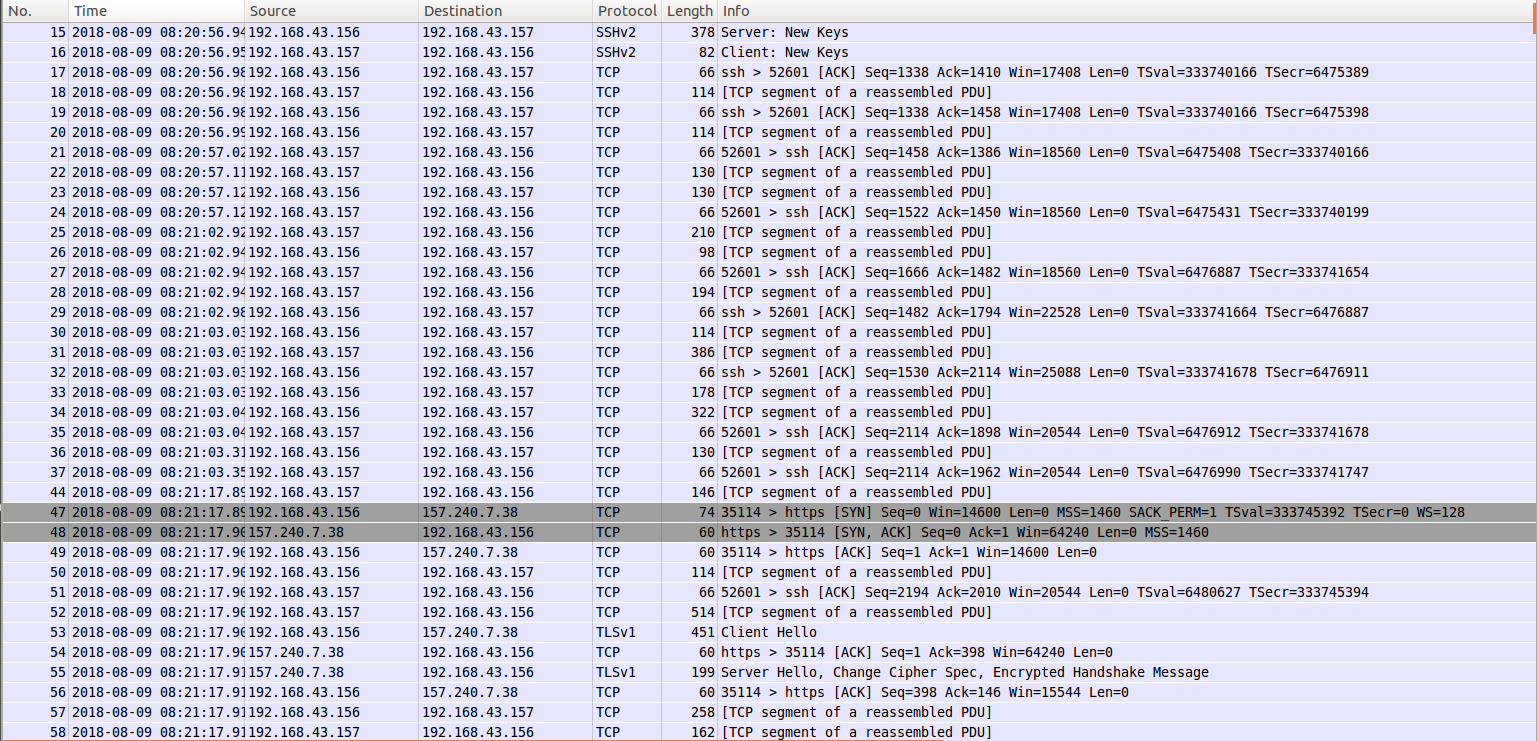
\includegraphics[width=1\linewidth]{Wiresharkfacebook}
\caption{Proxy Packet Transfer}
\label{fig:wiresharkfacebook}
\end{figure}

\noindent \textbf{Question 4:}\\
If \texttt{ufw} blocks SSH TCP port 22, can a SSH tunnel still be set up to evade egress filtering?\\
\\\textbf{Answer 4:}\\
Yes. Both on the server and client side, the port number for SSH can be changed by modifying the file \texttt{/etc/ssh/sshd\_config}. For this example, the port number is changed from 22 to 26. The SSH service is then restarted and tested. For convenience, the \texttt{-p} switch is sufficient to show that a SSH tunnel can be established.

\begin{figure}[H]
\centering
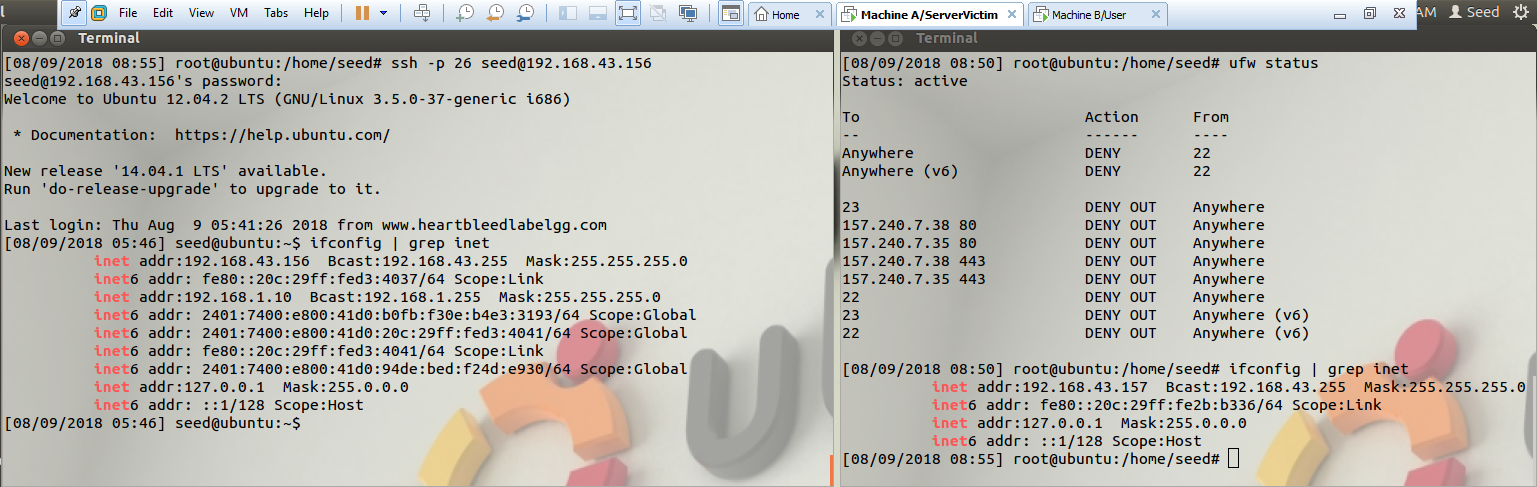
\includegraphics[width=0.8\linewidth]{SSHegressbypass}
\caption{SSH Egress Filtering Bypassed}
\label{fig:sshegressbypass}
\end{figure}

\noindent Again, we see from the figure above that we can obtain a connection to a remote server and obtain the server's IP address, bypassing the \texttt{ufw} firewall.
\subsection{Web Proxy -- Application Firewall}
Application firewalls are another type of firewall that can be used to filter packets. Instead of inspecting data at the layer data (looking at the header fields of the packets), these firewalls look at application-layer data. These firewalls control access from/to applications or services. 

\subsubsection{\texttt{squid} Server Setup}
A common implementation of this firewall are web proxies. For this lab, the web proxy that will be used is \texttt{squid} and can be installed by executing \texttt{sudo apt-get squid}.\\\\After installation, the firewall policies can be set-up by modifying the file \texttt{squid.conf} in the folder \texttt{/etc/squid3}. The \texttt{squid} server needs to be restarted every time a modification has been done to the file, otherwise the new rules will not effect.\\\\Two VMs are set-up for this task, Machine A and B. Machine A will emulate the system that requires its browsing restricted and Machine B will run the web proxy. To configure the browser for Machine A, the ``HTTP Proxy'' option is set to Machine B's IP address and port 3128 (default port for \texttt{squid} service).

\begin{figure}[H]
\centering
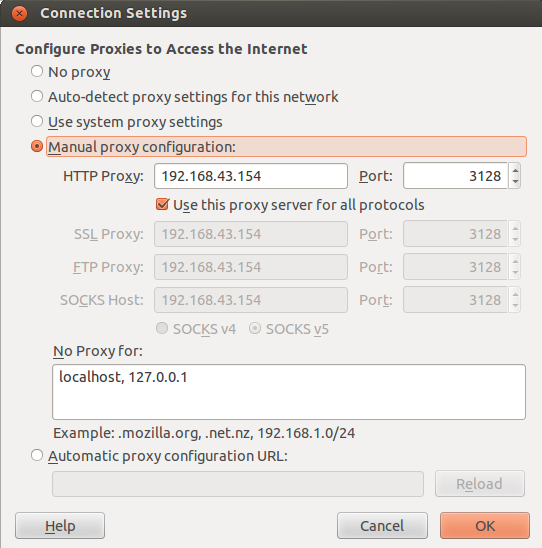
\includegraphics[width=0.7\linewidth]{FFProxyConf}
\caption{Proxy Configuration Settings}
\label{fig:ffproxyconf}
\end{figure}
\noindent After configuration, any website that is visited will show an access denied error. Also, we notice that at the footer that \texttt{squid} and the version of the software is mentioned when the site is blocked. This shows that the configuration of the software is correct and that all sites are blocked by default after installing \texttt{squid}.

\begin{figure}[H]
\centering
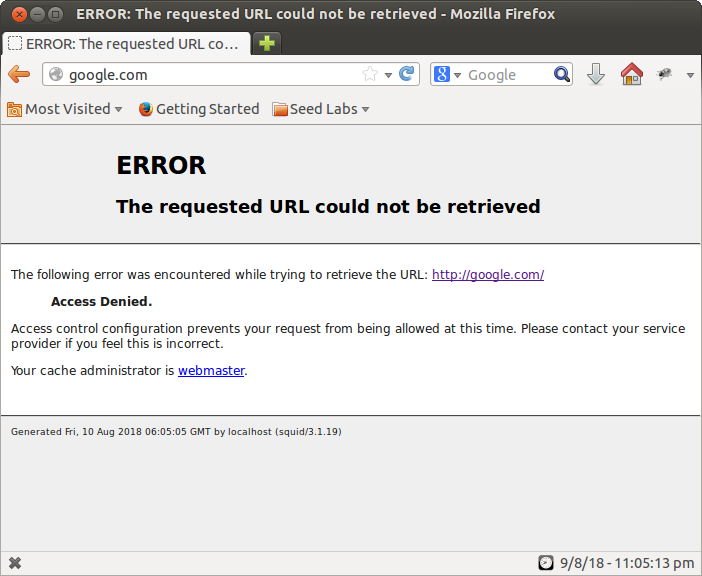
\includegraphics[width=0.7\linewidth]{squidblock}
\caption{Blocked By Proxy}
\label{fig:squidblock}
\end{figure}
\noindent To check why all sites are blocked, the configuration file needs to be accessed. To find the line causing this quickly, this line is used.
\begin{verbatim}
$ cat /etc/squid3/squid.conf | grep deny
\end{verbatim}
\noindent The lines that stands out from the printed result are in the firewall access block of code. In this block, every site is denied with the exception of localhost sites, which are not affected.
\begin{verbatim}
http_access deny manager
http_access deny !Safe_ports
http_access deny CONNECT !SSL_ports
#http_access deny to_localhost
# And finally deny all other access to this proxy
http_access deny all
\end{verbatim}
To allow all websites through the web proxy, an Access Control List (ACL) needs to be created. By doing so, we can allow this ACL to access any website. The following lines must be added \textbf{before} \texttt{http\_access deny all}.
\begin{verbatim}
acl all src 0.0.0.0/0   #acl <acl name> <type> <data>
http_access allow all   #http_access <allow/deny> <acl name>
\end{verbatim}
\noindent To allow specific sites like \texttt{google.com} to be accessed and other sites blocked, the ACL needs to be used. The previous entries need to be commented out or it will conflict with the current ACL.
\begin{verbatim}
#acl all src 0.0.0.0/0
#http_access allow all
acl google dstdomain .google.com.
http_access allow google
\end{verbatim}

\begin{figure}[H]
\begin{subfigure}{0.45\textwidth}
\centering
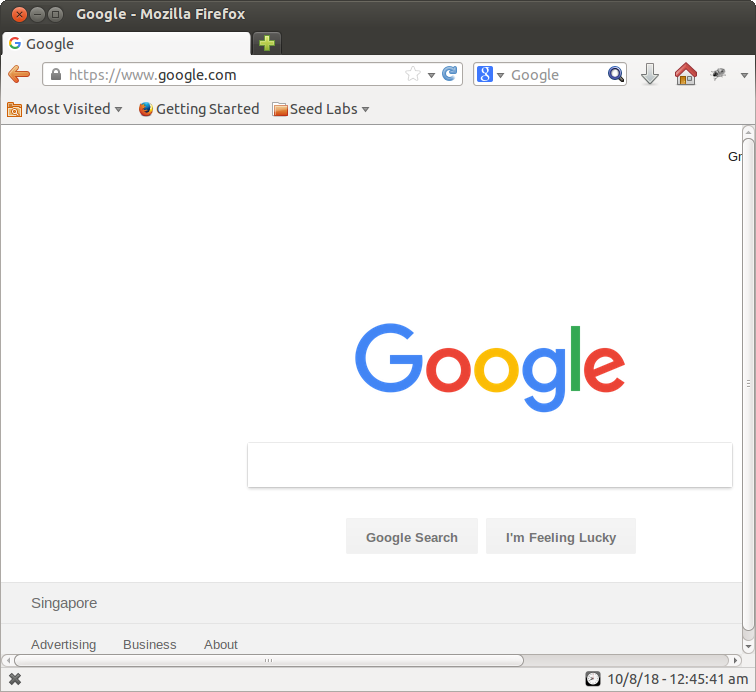
\includegraphics[width=0.95\linewidth]{gaccess}
\caption{Access to Google}
\label{fig:blockaccess}
\end{subfigure}
~
\begin{subfigure}{0.45\textwidth}
\centering
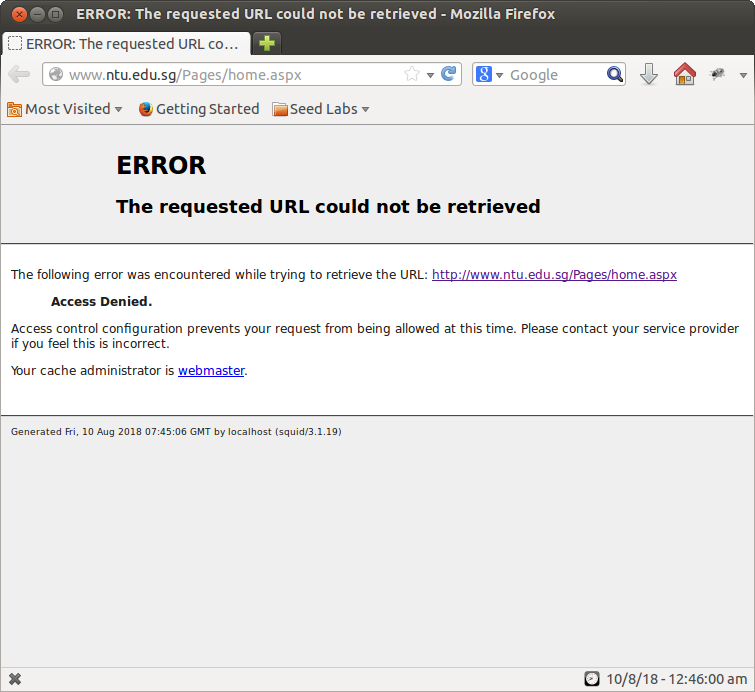
\includegraphics[width=0.95\linewidth]{blockaccess}
\caption{Blocked to Anywhere Else}
\label{fig:gaccess}
\end{subfigure}
\caption{Selective Access via ACL}
\end{figure}
\noindent Analysing the captured packets via Wireshark, we noticed that for Google the packet flow was the same as when SSH was used. The data is passed from Machine A to the web proxy and that data was forwarded to the respective destination IP address and port. Similarly, return of data from the destination goes through the web proxy and back to Machine A.\\\\However, for the site that was denied, the data goes through from Machine A to the web proxy but is now returned an access denied page. This is in contrast to the previous firewall where the packets are dropped.
\subsubsection{Firewall Evasion}
\textbf{Question 5:}\\If \texttt{ufw} blocks TCP port 3128, can the web proxy still be used to evade the firewall?\\\\\textbf{Answer 5:}\\Yes. Similar to the SSH tunnel, the listening port for the \texttt{squid} server can still be changed to some arbitrary port number. To show that this is possible, an entry in the \texttt{ufw} firewall is added to block any packets to destination port 3128.
\begin{verbatim}
$ sudo ufw deny out 3128/tcp
$ sudo ufw disable
$ sudo ufw enable 
\end{verbatim}
\noindent A random port number is selected, for this scenario the port number is amended to 10000. Port numbers below 1024 are usually reserved for specific applications and it is highly advisable to not use that range.\\\\
In the \texttt{squid.conf} file, the line \texttt{http\_port} is searched for (\texttt{Ctrl + W} in nano) and modified.\\\\
\texttt{http\_port 3128 $\rightarrow$ http\_port 10000}\\\\
The \texttt{squid} service is restarted and the browser is configured to use port 10000 also.

\begin{figure}[H]
\begin{subfigure}{1\textwidth}
\centering
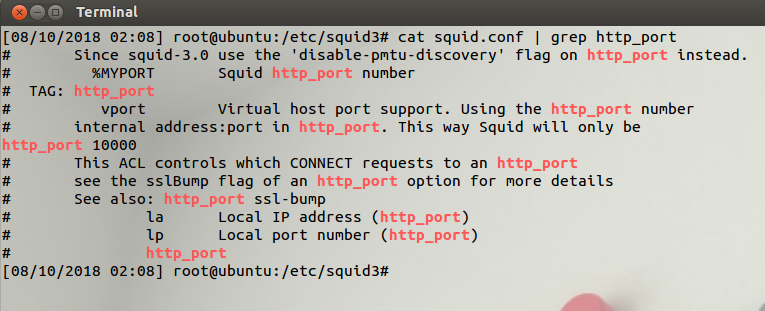
\includegraphics[width=0.95\linewidth]{portconf}
\caption{\texttt{squid} Port Configuration}
\label{fig:squidport}
\end{subfigure}
\\
\begin{subfigure}{1\textwidth}
\centering
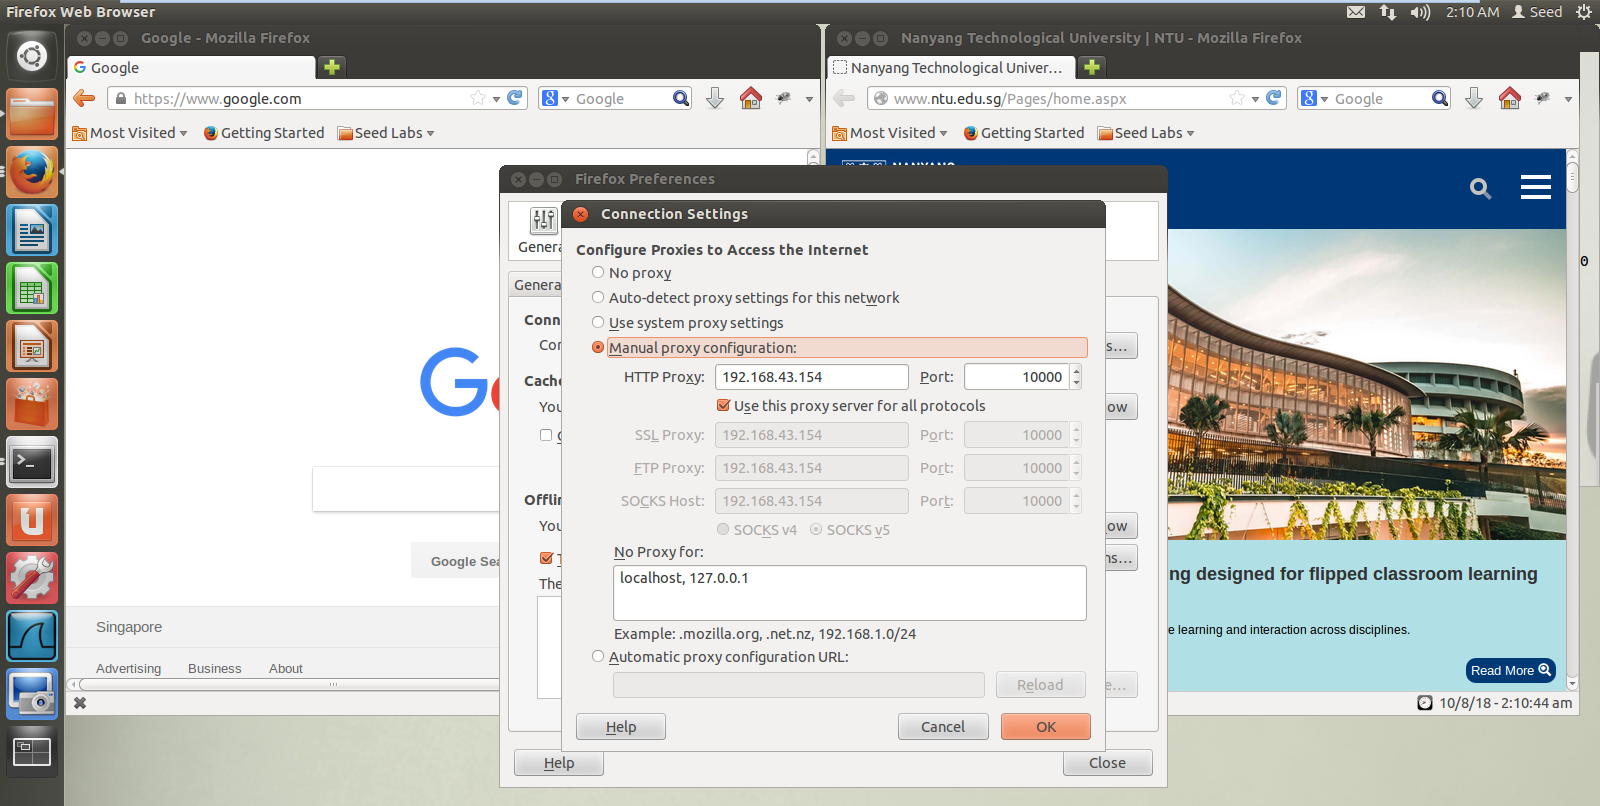
\includegraphics[width=0.95\linewidth]{accessbypass}
\caption{Access Re-established}
\label{fig:bypasssquid}
\end{subfigure}
\caption{Firewall Bypassed}
\end{figure}
\subsection{URL Rewriting/Redirection}
\subsubsection{\texttt{myprog.pl}}
Apart from acting as a firewall, \texttt{squid} can also be used to rewrite URLs to redirect users to another web site. This can be done using any type of programming language. A perl program \texttt{myprog.pl} has been provided to demonstrate URL rewriting capabilities. It has been attached to \hyperref[ch:AppB]{Appendix B}.\\\\In short, the code checks whether the URL entered is identical to \texttt{www.ntu.edu.sg}. If it is, then the user is redirected to \texttt{www.google.com.sg}. The operator \texttt{=\~} is used to check if the string is identical and not exact/equal (\texttt{==}).\\\\To attach the the program to \texttt{squid}, the following lines are added to the \texttt{squid.conf} file.
\begin{verbatim}
url_rewrite_program /home/seed/myprog.pl #Location of file
url_rewrite_children 5
\end{verbatim}
The perl file must be marked as executable (using \texttt{chmod +x}) or the firewall will not work. In the event the file cannot be found by \texttt{squid}, the URL rewrite program can be placed in \texttt{/etc/squid3} instead. \\\\
As previously mentioned, any attempt to view the site \texttt{www.ntu.edu.sg} will redirect the user to \texttt{www.google.com.sg}. The packets from this action are captured in Wireshark and analysed in detail. In particular, we look into the initial packet that was sent over the wire to the server and follow the packet stream. This action can be done by right-clicking the corresponding packet and selecting the option ``Follow TCP Stream''. The data printed shows that the web proxy replies with a ``HTTP 302 Moved Temporarily'' and the rewritten URL response instead of forwarding the response to our intended destination.

\begin{figure}[H]
\centering
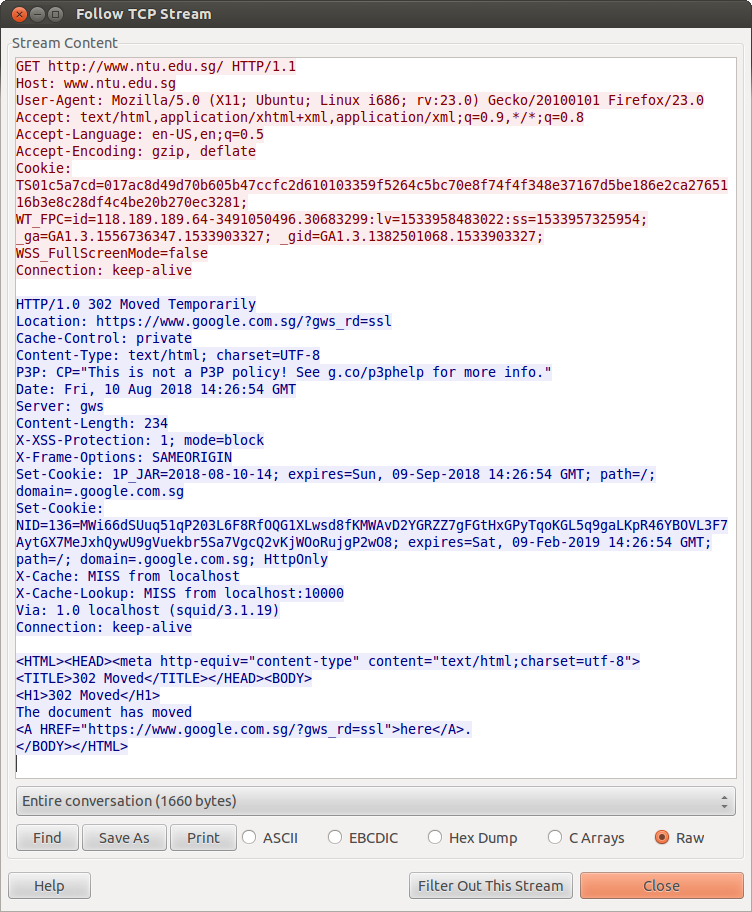
\includegraphics[width=0.7\linewidth]{tcpstream}
\caption{TCP Stream Data}
\label{fig:tcpstream}
\end{figure}
\subsubsection{Replace Facebook Pages With Stop Sign}
In this lab instead of redirecting users from a legitimate site to another, we redirect users from Facebook to a big red stop sign to act as a deterrent to prevent users from being distracted. The same program is used with some modifications and it has been reflected in \hyperref[ch:AppBStop]{Appendix B}.\\\\Again, typing \texttt{facebook.com} into the browser will force a redirection to a stop sign. This is evident if the TCP stream was followed in Wireshark.

\begin{figure}[H]
\centering
\begin{subfigure}{0.48\textwidth}
\centering
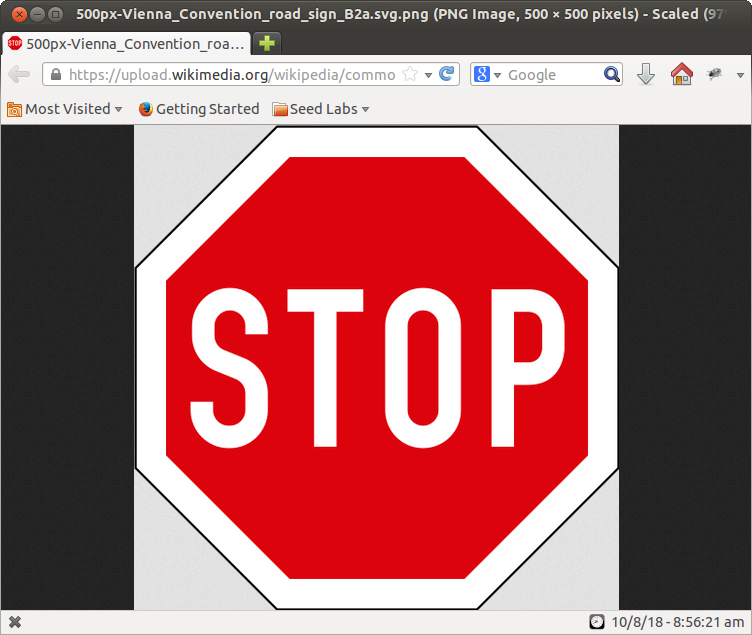
\includegraphics[width=1\linewidth]{stopsign}
\caption{Facebook Redirect}
\label{fig:stopsign}
\end{subfigure}
~
\begin{subfigure}{0.48\textwidth}
\centering
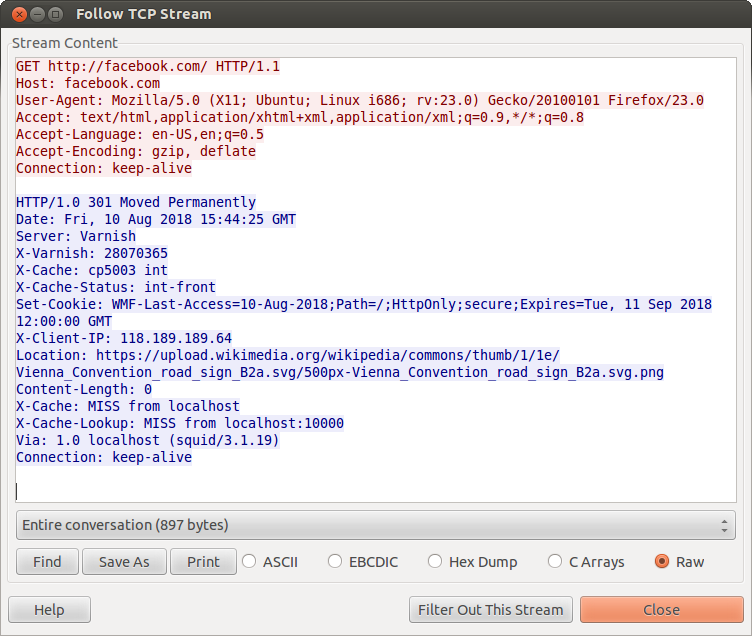
\includegraphics[width=1\linewidth]{facebookstop}
\caption{Stream Capture}
\label{fig:facebookstop}
\end{subfigure}
\caption{Image Redirect}
\end{figure}
\subsubsection{Replacing All Images In A Page}
This part will look at replacing all images on a web page with an image of our choice. When an image is loaded on the page, it will immediately send a URL request for each image. These URLs will be identified and replaced accordingly by the web proxy. The provided code again has been attached to \hyperref[ch:AppBImgMod]{Appendix B}.\\\\A site that has multiple images is accessed, such as the NTU homepage. All images that end with any mentioned image extension (in the code) will have it replaced by a stop sign. This is evident as all the images have been replaced, such as shown in the figure below.
\begin{figure}[H]
\centering
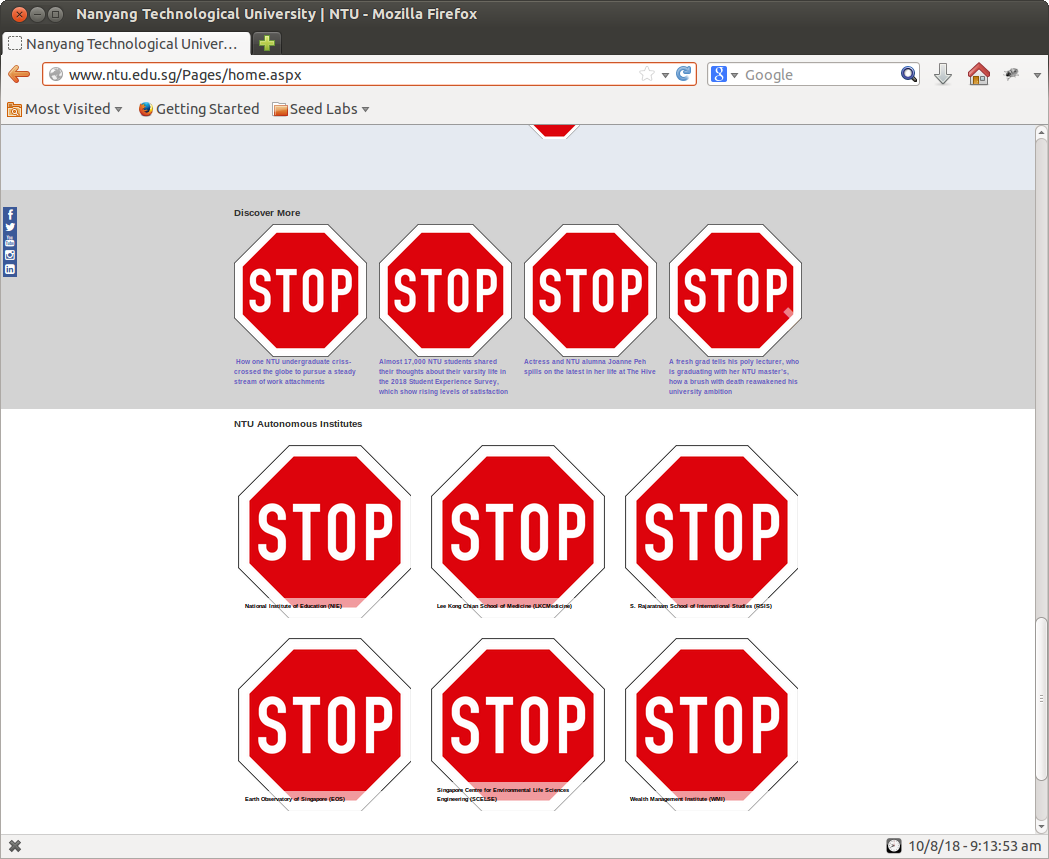
\includegraphics[width=0.9\linewidth]{ntudeface}
\caption{NTU Defaced via Web Proxy URL Rewriting (Zoomed out to 30\%)}
\label{fig:ntudeface}
\end{figure}
\noindent The figure shown above shows how powerful web proxies can be used to deface websites and redirect as well as to control access to websites, shown in the previous sections. Programs and proxies can also be adapted to evade filtering on any level or to inject malicious code into websites where the user is not aware of.

\newpage
\section{Appendix A}
\label{ch:AppA}
\subsection{Packet Filtering Module -- pfm.c}
\begin{minted}[linenos,breaklines]{C}
#include <linux/kernel.h>
#include <linux/module.h>
#include <linux/netfilter.h>
#include <linux/netfilter_ipv4.h>
#include <linux/ip.h>
#include <linux/in.h>

static struct nf_hook_ops nfho;         //struct holding set of hook function options
struct iphdr *iphd;

//function to be called by hook
unsigned int hook_func(unsigned int hooknum, struct sk_buff *skb, const struct net_device *in, const struct net_device *out, int (*okfn)(struct sk_buff *))
{
  iphd = ip_hdr(skb);
  if(iphd->protocol ==IPPROTO_ICMP){		//Checks for ICMP packet (Added from original)
  	printk(KERN_INFO "packet dropped\n");   //log to var/log/messages
  	return NF_DROP;                         //drops the packet
	}
  else	//Accept if not ICMP (Added from original)
	return NF_ACCEPT;
}

//Called when module loaded using 'insmod'
int init_module()
{
  nfho.hook = &hook_func;              //function to call when conditions below met
  nfho.hooknum = NF_INET_PRE_ROUTING;  //called right after packet recieved, first hook in Netfilter
  nfho.pf = PF_INET;                   //IPV4 packets
  nfho.priority = NF_IP_PRI_FIRST;     //set to highest priority over all other hook functions
  nf_register_hook(&nfho);             //register hook

  return 0;                            //return 0 for success
}

//Called when module unloaded using 'rmmod'
void cleanup_module()
{
  nf_unregister_hook(&nfho);                     //cleanup – unregister hook
}
\end{minted}
\noindent *Notes for the code above:
\begin{enumerate}
\item The \texttt{\&} symbol is missing from the original documentation and will cause the system to crash when the module is added to the kernel. The function definition found in \texttt{netfilter.h} explictly provides the structure for \texttt{nf\_hook\_ops} has been provided below.
\begin{minted}{C}
struct nf_hook_ops {
	struct list_head list;

	/* User fills in from here down. */
	nf_hookfn *hook;
	struct module *owner;
	u_int8_t pf;
	unsigned int hooknum;
	/* Hooks are ordered in ascending priority. */
	int priority;
};
\end{minted}
\item The function definition for the hook function has an added \texttt{*} for \texttt{*skb} when compared to the \texttt{netfilter.h} file and has been removed (although it can be simply corrected by using \texttt{ip\_hdr(*skb)} on line 14).
\begin{minted}{C}
typedef unsigned int nf_hookfn(unsigned int hooknum,
			       struct sk_buff *skb,
			       const struct net_device *in,
			       const struct net_device *out,
			       int (*okfn)(struct sk_buff *));
\end{minted}
\end{enumerate}
\subsection{Makefile}
\begin{minted}[linenos]{bash}
obj-m += pfm2.o

all:
        make -C /lib/modules/$(shell uname -r)/build M=$(PWD) modules

clean:
        make -C /lib/modules/$(shell uname -r)/build M=$(PWD) clean
\end{minted}
\section{Appendix B}
\label{ch:AppB}
\subsection{\texttt{myprog.pl}}
\begin{minted}[linenos,breaklines]{perl}
#!/usr/bin/perl -w
use strict;
use warnings;

# Forces a flush after every write or print on the STDOUT
select STDOUT; $| =1;

# Get the input line by line from the standard input.
# Each line contains a URL and some other information.
while (<>)
{
	my @parts = split;
	my $url = $parts[0];
	# If you copy and paste this code from this PDF file,
	# the ~ (tilde) character may not be copied correctly.
	# Remove it, and then type the character manually.
	if ($url =~ /www\.ntu\.edu\.sg/) {
		#URL Rewriting
		print "http://www.google.com.sg\n";
	}
	else {
		# No Rewriting
		print "\n";
	}
}
\end{minted}
\subsection{\texttt{myprog.pl} -- Stop Sign}
\label{ch:AppBStop}
\begin{minted}[linenos,breaklines]{perl}
#!/usr/bin/perl -w
use strict;
use warnings;

# Forces a flush after every write or print on the STDOUT
select STDOUT; $| = 1;

# Get the input line by line from the standard input.
# Each line contains a URL and some other information.
while (<>)
{
	my @parts = split;
	my $url = $parts[0];
	#If you copy and paste this code from this PDF file,
	# the ~ (tilde) character may not be copied correctly.
	# Remove it, and then type the character manually.
	if ($url =~ /facebook\.com/){
		#URL Rewriting
		print "http://upload.wikimedia.org/wikipedia/commons/ thumb/1/1e/Vienna_Convention_road_sign_B2a.svg/ 500px-Vienna_Convention_road_sign_B2a.svg.png\n";
	}
	else {
		#No Rewriting
		print "\n";
	}
}
\end{minted}
*Note: Using \texttt{https} for the URL redirect will cause \texttt{squid} to identify it as an invalid protocol and will stop the redirection with an error message.
\subsection{\texttt{myprog.pl} -- Image Manipulation}
\label{ch:AppBImgMod}
\begin{minted}[linenos,breaklines]{perl}
#!/usr/bin/perl -w
use strict;
use warnings;

# Forces a flush after every write or print on the STDOUT
select STDOUT; $| = 1;

# Get the input line by line from the standard input.
# Each line contains a URL and some other information.
while (<>)
{
    my @parts = split;
    my $url = $parts[0];
    #If you copy and paste this code from this PDF file,
    # the ~ (tilde) character may not be copied correctly.
    # Remove it, and then type the character manually.
    if ($url =~ /\.(jpg|png|svg|PNG|JPG|JPEG|BMP|bmp|jpeg|SVG)/){
            #URL Rewriting
            print "http://upload.wikimedia.org/wikipedia/commons/ thumb/1/1e/Vienna_Convention_road_sign_B2a.svg/ 500px-Vienna_Convention_road_sign_B2a.svg.png\n";
    }
    else {
            #No Rewriting
            print "\n";
    }
}

\end{minted}
\end{document}